% Very simple template for lab reports. Most common packages are already included.
\documentclass[a4paper, 11pt]{article}
\usepackage[utf8]{inputenc} % Change according your file encoding
\usepackage{graphicx}
\usepackage{url}
\usepackage{xcolor}
\usepackage{colortbl}
\usepackage{array}
\usepackage{tikz}

% Define the color gradient
\definecolor{darkgreen}{RGB}{26, 188, 156}
\definecolor{medgreen}{RGB}{52, 211, 153}
\definecolor{lightgreen}{RGB}{132, 204, 22}
\definecolor{yellow}{RGB}{250, 204, 21}
\definecolor{orange}{RGB}{251, 146, 60}
\definecolor{red}{RGB}{239, 68, 68}

%opening
\title{Report X: Homework Report Template}
\author{Your name}
\date{\today{}}

\begin{document}

\maketitle

\section{Introduction}

\textit{Summary of the work you've done, what are the topics we cover
  in this seminar, etc. Remember that you should deliver this report
  at the start of the seminar.}

What is the main topic related to distributed systems covered in this seminar?
Why is it important?

\begin{figure}[htbp]
  \centering
  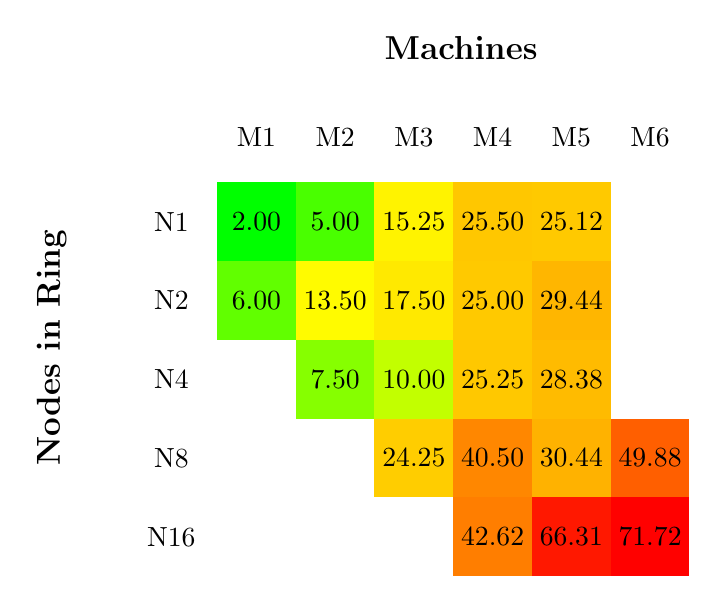
\begin{tikzpicture}[scale=0.8]
    % Label: "Machines" above columns
    \node[font=\large\bfseries] at (4.5, 1.5) {Machines};
    
    % Label: "Nodes in Ring" to the left of rows
    \node[font=\large\bfseries, rotate=90] at (-2, -3.25) {Nodes in Ring};
    
    \foreach \y [count=\n] in {
      {2.00,5.00,15.25,25.50,25.12, },
      {6.00,13.50,17.50,25.00,29.44, },
      { ,7.50,10.00,25.25,28.38, },
      { , ,24.25,40.50,30.44,49.88},
      {, , ,42.62,66.31,71.72},
      } {
        % column labels
        \ifnum\n<10
          \node[minimum size=10mm] at (1.25*\n, 0.1) {M\n};
        \fi
        % heatmap tiles
        \foreach \x [count=\m] in \y {
          \ifx\x\empty
            % Empty cell - fill with white
            \node[fill=white, minimum size=10mm, inner sep=0pt, outer sep=0pt] 
                  at (1.25*\m,-1.25*\n) {};
          \else
            % Data cell - calculate color
            \pgfmathsetmacro{\normalized}{(\x-2)/(72-2)}
            \pgfmathparse{\normalized<0.15?1:0}
            \ifnum\pgfmathresult=1
              % Low values (0-0.15): green to yellow (very fast transition)
              \pgfmathsetmacro{\r}{\normalized*6.667}
              \pgfmathsetmacro{\g}{1}
              \pgfmathsetmacro{\b}{0}
              \definecolor{cellcolor}{rgb}{\r,\g,\b}
            \else
              % High values (0.15-1): yellow to red
              \pgfmathsetmacro{\r}{1}
              \pgfmathsetmacro{\g}{(1-\normalized)*1.176}
              \pgfmathsetmacro{\b}{0}
              \definecolor{cellcolor}{rgb}{\r,\g,\b}
            \fi
            \node[fill=cellcolor, 
                  minimum size=10mm, text=black, inner sep=0pt, outer sep=0pt] 
                  at (1.25*\m,-1.25*\n) {\x};
          \fi
        }
      }
    % row labels
    \foreach \a [count=\i] in {1, 2, 4, 8, 16} {
      \node[minimum size=10mm] at (-0.1,-1.25*\i) {N\a};
    }
  \end{tikzpicture}
  \caption{TODO: make second subchart}
  \label{fig:heatmap}
\end{figure}

\section{Main problems and solutions}

\textit{Summarize your problems, proposed solutions, etc. You do not
  need to copy\&paste your code. Only if needed, you may write down
  small code snipeds to show how you have solved a specific
  problem/question.}

Did you find any specific problem with the development of your
solution?  How did you solve it?

If you want to give a code example you can do it uing the verbatim environment.
\begin{verbatim}
this(X) ->
    Y = is(X),
    a(test(Y)).
\end{verbatim}

\section{Evaluation}

\textit{If needed, you may provide figures or tables with main results
  evaluating your proposals. For each seminar, we will provide you
  with some guidance on which kind of evaluation you should do.}


And Figures \ref{fig:results1} and \ref{fig:results2 } shows how to
add a figure with some results. These figures have been created with
gnuplot. There are tons of different kinds of plots that can be
generated with gnuplot. Make sure to check out
\url{http://gnuplot.info/demo/} and look at them so you can see what
can you do with this program.


To obtain these figures you have to:
\begin{enumerate}

\item Create the data file from the experiments (look at file
  experiment.dat)

\item Create a gnuplot file to create a figure in eps format (look at
  files results1.plot and results2.plot). These files may be very
  complex. But for the results we want to show, these examples are
  enough. To create the eps figures, execute in terminal:

\begin{verbatim}
$> gnuplot results1.plot 
\end{verbatim}

\item As pdflatex does not recognize eps files, you must convert them
  to pdf files. This is done by (it will generate a file
  results1.pdf):

\begin{verbatim}
$> epstopdf results1.eps
\end{verbatim}

\item That's it! Just include the figure as shown in this template and
  compile the latex as explained in the document ``Introduction to
  \LaTeXe''.

\end{enumerate}


If you want, you can also create a table of results as Table
\ref{tab:results}. If you look at the template code, you will see how
to do a table in \LaTeX.

\begin{table}[h]
\centering
\begin{tabular}{lcc}
First column & Second column & Third column\\\hline
Case 1 & 1.1 & 1.2\\\hline
Case 2 & 2.1 & 2.2\\\hline
Case 3 & 3.1 & 3.2\\\hline
\end{tabular}
\caption{Some random results in a table}
\label{tab:results}
\end{table}

\section{Conclusions}

\textit{Change the layout of this template as you want. It's only for
  your guidance but if you feel that you need a different structure,
  feel free to change it. The report should not be too long ($\approx$
  2-3 pages).}

What have you learnt from the problem presented?
Was it useful?


\end{document}
